\documentclass[twoside,openright,titlepage,numbers=noenddot,headinclude,%
               footinclude=true,cleardoublepage=empty,abstractoff,BCOR=5mm,%
               paper=a4,fontsize=11pt,ngerman,american]{scrreprt}

% Custom config ===============================================================

% Classic thesis
\usepackage{amssymb}
% ****************************************************************************************************
% classicthesis-config.tex
% formerly known as loadpackages.sty, classicthesis-ldpkg.sty, and classicthesis-preamble.sty
% Use it at the beginning of your ClassicThesis.tex, or as a LaTeX Preamble
% in your ClassicThesis.{tex,lyx} with % ****************************************************************************************************
% classicthesis-config.tex
% formerly known as loadpackages.sty, classicthesis-ldpkg.sty, and classicthesis-preamble.sty
% Use it at the beginning of your ClassicThesis.tex, or as a LaTeX Preamble
% in your ClassicThesis.{tex,lyx} with % ****************************************************************************************************
% classicthesis-config.tex
% formerly known as loadpackages.sty, classicthesis-ldpkg.sty, and classicthesis-preamble.sty
% Use it at the beginning of your ClassicThesis.tex, or as a LaTeX Preamble
% in your ClassicThesis.{tex,lyx} with \input{classicthesis-config}
% ****************************************************************************************************
% If you like the classicthesis, then I would appreciate a postcard.
% My address can be found in the file ClassicThesis.pdf. A collection
% of the postcards I received so far is available online at
% http://postcards.miede.de
% ****************************************************************************************************

% ****************************************************************************************************
% 1. Configure classicthesis for your needs here, e.g., remove "drafting" below
% in order to deactivate the time-stamp on the pages
% ****************************************************************************************************
\PassOptionsToPackage{listings,%drafting,% %eulerchapternumbers,%
				 pdfspacing,eulermath,%floatperchapter,%linedheaders,%
				 subfig,parts,dottedtoc}{classicthesis}
% ********************************************************************
% Available options for classicthesis.sty
% (see ClassicThesis.pdf for more information):
% drafting
% parts nochapters linedheaders
% eulerchapternumbers beramono eulermath pdfspacing minionprospacing
% tocaligned dottedtoc manychapters
% listings floatperchapter subfig
% ********************************************************************

% ********************************************************************
% Triggers for this config
% ********************************************************************
\usepackage{ifthen}
\newboolean{enable-backrefs} % enable backrefs in the bibliography
\setboolean{enable-backrefs}{false} % true false
% ****************************************************************************************************


% ****************************************************************************************************
% 2. Personal data and user ad-hoc commands
% ****************************************************************************************************
\newcommand{\myTitle}{Identifing At Risk Students\xspace}
\newcommand{\mySubtitle}{A Supervised Learning Project\xspace}
%\newcommand{\myDegree}{Doktor-Ingenieur (Dr.-Ing.)\xspace}
\newcommand{\myName}{Omoju Miller\xspace}
%\newcommand{\myProf}{Put name here\xspace}
%\newcommand{\myOtherProf}{Put name here\xspace}
%\newcommand{\mySupervisor}{Pierre Geurts\xspace}
%\newcommand{\myFaculty}{Faculty of Applied Sciences\xspace}
%\newcommand{\myDepartment}{Department of EE and CS\xspace}
%\newcommand{\myUni}{University of Liege\xspace}
%\newcommand{\myLocation}{Liege, Belgium\xspace}
%\newcommand{\myTime}{June 2014\xspace}
\newcommand{\myVersion}{version 1.0\xspace}

% ********************************************************************
% Setup, finetuning, and useful commands
% ********************************************************************
\newcounter{dummy} % necessary for correct hyperlinks (to index, bib, etc.)
\newlength{\abcd} % for ab..z string length calculation
\providecommand{\mLyX}{L\kern-.1667em\lower.25em\hbox{Y}\kern-.125emX\@}
\newcommand{\ie}{i.\,e.}
\newcommand{\Ie}{I.\,e.}
\newcommand{\eg}{e.\,g.}
\newcommand{\Eg}{E.\,g.}
% ****************************************************************************************************


% ****************************************************************************************************
% 3. Loading some handy packages
% ****************************************************************************************************
% ********************************************************************
% Packages with options that might require adjustments
% ********************************************************************
%\PassOptionsToPackage{latin9}{inputenc}	% latin9 (ISO-8859-9) = latin1+"Euro sign"
% \usepackage{inputenc}

\usepackage[applemac]{inputenc}

%\PassOptionsToPackage{ngerman,american}{babel}   % change this to your language(s)
% Spanish languages need extra options in order to work with this template
%\PassOptionsToPackage{spanish,es-lcroman}{babel}
 \usepackage{babel}

\PassOptionsToPackage{square,authoryear}{natbib}
 \usepackage{natbib}

\PassOptionsToPackage{fleqn}{amsmath}		% math environments and more by the AMS
 \usepackage{amsmath}

% ********************************************************************
% General useful packages
% ********************************************************************
\PassOptionsToPackage{T1}{fontenc} % T2A for cyrillics
	\usepackage{fontenc}


\usepackage{lipsum}
\usepackage{textcomp} % fix warning with missing font shapes
%\usepackage{scrhack} % fix warnings when using KOMA with listings package
\usepackage{xspace} % to get the spacing after macros right
\usepackage{mparhack} % get marginpar right
%\usepackage{fixltx2e} % fixes some LaTeX stuff
\PassOptionsToPackage{printonlyused,smaller}{acronym}
	\usepackage{acronym} % nice macros for handling all acronyms in the thesis
%\renewcommand*{\acsfont}[1]{\textssc{#1}} % for MinionPro
%\renewcommand{\bflabel}[1]{{#1}\hfill} % fix the list of acronyms
% ****************************************************************************************************


% ****************************************************************************************************
% 4. Setup floats: tables, (sub)figures, and captions
% ****************************************************************************************************
\usepackage{tabularx} % better tables
	\setlength{\extrarowheight}{3pt} % increase table row height
\newcommand{\tableheadline}[1]{\multicolumn{1}{c}{\spacedlowsmallcaps{#1}}}
\newcommand{\myfloatalign}{\centering} % to be used with each float for alignment
\usepackage{caption}
\captionsetup{format=hang,font=small}
\usepackage{subfig}
% ****************************************************************************************************


% ****************************************************************************************************
% 5. Setup code listings
% ****************************************************************************************************
\usepackage{listings}
%\lstset{emph={trueIndex,root},emphstyle=\color{BlueViolet}}%\underbar} % for special keywords
\lstset{language=[LaTeX]Tex,%C++,
    keywordstyle=\color{RoyalBlue},%\bfseries,
    basicstyle=\small\ttfamily,
    %identifierstyle=\color{NavyBlue},
    commentstyle=\color{Green}\ttfamily,
    stringstyle=\rmfamily,
    numbers=none,%left,%
    numberstyle=\scriptsize,%\tiny
    stepnumber=5,
    numbersep=8pt,
    showstringspaces=false,
    breaklines=true,
    frameround=ftff,
    frame=single,
    belowcaptionskip=.75\baselineskip
    %frame=L
}
% ****************************************************************************************************


% ****************************************************************************************************
% 6. PDFLaTeX, hyperreferences and citation backreferences
% ****************************************************************************************************
% ********************************************************************
% Using PDFLaTeX
% ********************************************************************
\PassOptionsToPackage{pdftex,hyperfootnotes=true,pdfpagelabels}{hyperref}
	\usepackage{hyperref}  % backref linktocpage pagebackref
\pdfcompresslevel=9
\pdfadjustspacing=1
\PassOptionsToPackage{pdftex}{graphicx}
	\usepackage{graphicx}

% ********************************************************************
% Setup the style of the backrefs from the bibliography
% (translate the options to any language you use)
% ********************************************************************
\newcommand{\backrefnotcitedstring}{\relax}%(Not cited.)
\newcommand{\backrefcitedsinglestring}[1]{(Cited on page~#1.)}
\newcommand{\backrefcitedmultistring}[1]{(Cited on pages~#1.)}
\ifthenelse{\boolean{enable-backrefs}}%
{%
		\PassOptionsToPackage{hyperpageref}{backref}
		\usepackage{backref} % to be loaded after hyperref package
		   \renewcommand{\backreftwosep}{ and~} % separate 2 pages
		   \renewcommand{\backreflastsep}{, and~} % separate last of longer list
		   \renewcommand*{\backref}[1]{}  % disable standard
		   \renewcommand*{\backrefalt}[4]{% detailed backref
		      \ifcase #1 %
		         \backrefnotcitedstring%
		      \or%
		         \backrefcitedsinglestring{#2}%
		      \else%
		         \backrefcitedmultistring{#2}%
		      \fi}%
}{\relax}

% ********************************************************************
% Hyperreferences
% ********************************************************************
\hypersetup{%
    %draft,	% = no hyperlinking at all (useful in b/w printouts)
    colorlinks=true, linktocpage=true, pdfstartpage=3, pdfstartview=FitV,%
    % uncomment the following line if you want to have black links (e.g., for printing)
    %colorlinks=false, linktocpage=false, pdfborder={0 0 0}, pdfstartpage=3, pdfstartview=FitV,%
    breaklinks=true, pdfpagemode=UseNone, pageanchor=true, pdfpagemode=UseOutlines,%
    plainpages=false, bookmarksnumbered, bookmarksopen=true, bookmarksopenlevel=1,%
    hypertexnames=true, pdfhighlight=/O,%nesting=true,%frenchlinks,%
    urlcolor=webbrown, linkcolor=RoyalBlue, citecolor=webgreen, %pagecolor=RoyalBlue,%
    %urlcolor=Black, linkcolor=Black, citecolor=Black, %pagecolor=Black,%
    pdftitle={\myTitle},%
    pdfauthor={\textcopyright\ \myName},%
    pdfsubject={},%
    pdfkeywords={},%
    pdfcreator={pdfLaTeX},%
    pdfproducer={LaTeX with hyperref and classicthesis}%
}

% ********************************************************************
% Setup autoreferences
% ********************************************************************
% There are some issues regarding autorefnames
% http://www.ureader.de/msg/136221647.aspx
% http://www.tex.ac.uk/cgi-bin/texfaq2html?label=latexwords
% you have to redefine the makros for the
% language you use, e.g., american, ngerman
% (as chosen when loading babel/AtBeginDocument)
% ********************************************************************
\makeatletter
\@ifpackageloaded{babel}%
    {%
       \addto\extrasamerican{%
					\renewcommand*{\figureautorefname}{Figure}%
					\renewcommand*{\tableautorefname}{Table}%
					\renewcommand*{\partautorefname}{Part}%
					\renewcommand*{\chapterautorefname}{Chapter}%
					\renewcommand*{\sectionautorefname}{Section}%
					\renewcommand*{\subsectionautorefname}{Section}%
					\renewcommand*{\subsubsectionautorefname}{Section}%
				}%
       \addto\extrasngerman{%
					\renewcommand*{\paragraphautorefname}{Absatz}%
					\renewcommand*{\subparagraphautorefname}{Unterabsatz}%
					\renewcommand*{\footnoteautorefname}{Fu\"snote}%
					\renewcommand*{\FancyVerbLineautorefname}{Zeile}%
					\renewcommand*{\theoremautorefname}{Theorem}%
					\renewcommand*{\appendixautorefname}{Anhang}%
					\renewcommand*{\equationautorefname}{Gleichung}%
					\renewcommand*{\itemautorefname}{Punkt}%
				}%
			% Fix to getting autorefs for subfigures right (thanks to Belinda Vogt for changing the definition)
			\providecommand{\subfigureautorefname}{\figureautorefname}%
    }{\relax}
\makeatother


% ****************************************************************************************************
% 7. Last calls before the bar closes
% ****************************************************************************************************
% ********************************************************************
% Development Stuff
% ********************************************************************
\listfiles
%\PassOptionsToPackage{l2tabu,orthodox,abort}{nag}
%	\usepackage{nag}
%\PassOptionsToPackage{warning, all}{onlyamsmath}
%	\usepackage{onlyamsmath}

% ********************************************************************
% Last, but not least...
% ********************************************************************
\usepackage{classicthesis}
% ****************************************************************************************************


% ****************************************************************************************************
% 8. Further adjustments (experimental)
% ****************************************************************************************************
% ********************************************************************
% Changing the text area
% ********************************************************************
%\linespread{1.05} % a bit more for Palatino
%\areaset[current]{312pt}{761pt} % 686 (factor 2.2) + 33 head + 42 head \the\footskip
%\setlength{\marginparwidth}{7em}%
%\setlength{\marginparsep}{2em}%

% ********************************************************************
% Using different fonts
% ********************************************************************
%\usepackage[oldstylenums]{kpfonts} % oldstyle notextcomp
%\usepackage[osf]{libertine}
%\usepackage{hfoldsty} % Computer Modern with osf
%\usepackage[light,condensed,math]{iwona}
%\renewcommand{\sfdefault}{iwona}
%\usepackage{lmodern} % <-- no osf support :-(
% \usepackage[T1]{fontenc}
% \usepackage{textcomp}
%\usepackage[urw-garamond]{mathdesign} <-- no osf support :-(
% ****************************************************************************************************

% ****************************************************************************************************
% If you like the classicthesis, then I would appreciate a postcard.
% My address can be found in the file ClassicThesis.pdf. A collection
% of the postcards I received so far is available online at
% http://postcards.miede.de
% ****************************************************************************************************

% ****************************************************************************************************
% 1. Configure classicthesis for your needs here, e.g., remove "drafting" below
% in order to deactivate the time-stamp on the pages
% ****************************************************************************************************
\PassOptionsToPackage{listings,%drafting,% %eulerchapternumbers,%
				 pdfspacing,eulermath,%floatperchapter,%linedheaders,%
				 subfig,parts,dottedtoc}{classicthesis}
% ********************************************************************
% Available options for classicthesis.sty
% (see ClassicThesis.pdf for more information):
% drafting
% parts nochapters linedheaders
% eulerchapternumbers beramono eulermath pdfspacing minionprospacing
% tocaligned dottedtoc manychapters
% listings floatperchapter subfig
% ********************************************************************

% ********************************************************************
% Triggers for this config
% ********************************************************************
\usepackage{ifthen}
\newboolean{enable-backrefs} % enable backrefs in the bibliography
\setboolean{enable-backrefs}{false} % true false
% ****************************************************************************************************


% ****************************************************************************************************
% 2. Personal data and user ad-hoc commands
% ****************************************************************************************************
\newcommand{\myTitle}{Identifing At Risk Students\xspace}
\newcommand{\mySubtitle}{A Supervised Learning Project\xspace}
%\newcommand{\myDegree}{Doktor-Ingenieur (Dr.-Ing.)\xspace}
\newcommand{\myName}{Omoju Miller\xspace}
%\newcommand{\myProf}{Put name here\xspace}
%\newcommand{\myOtherProf}{Put name here\xspace}
%\newcommand{\mySupervisor}{Pierre Geurts\xspace}
%\newcommand{\myFaculty}{Faculty of Applied Sciences\xspace}
%\newcommand{\myDepartment}{Department of EE and CS\xspace}
%\newcommand{\myUni}{University of Liege\xspace}
%\newcommand{\myLocation}{Liege, Belgium\xspace}
%\newcommand{\myTime}{June 2014\xspace}
\newcommand{\myVersion}{version 1.0\xspace}

% ********************************************************************
% Setup, finetuning, and useful commands
% ********************************************************************
\newcounter{dummy} % necessary for correct hyperlinks (to index, bib, etc.)
\newlength{\abcd} % for ab..z string length calculation
\providecommand{\mLyX}{L\kern-.1667em\lower.25em\hbox{Y}\kern-.125emX\@}
\newcommand{\ie}{i.\,e.}
\newcommand{\Ie}{I.\,e.}
\newcommand{\eg}{e.\,g.}
\newcommand{\Eg}{E.\,g.}
% ****************************************************************************************************


% ****************************************************************************************************
% 3. Loading some handy packages
% ****************************************************************************************************
% ********************************************************************
% Packages with options that might require adjustments
% ********************************************************************
%\PassOptionsToPackage{latin9}{inputenc}	% latin9 (ISO-8859-9) = latin1+"Euro sign"
% \usepackage{inputenc}

\usepackage[applemac]{inputenc}

%\PassOptionsToPackage{ngerman,american}{babel}   % change this to your language(s)
% Spanish languages need extra options in order to work with this template
%\PassOptionsToPackage{spanish,es-lcroman}{babel}
 \usepackage{babel}

\PassOptionsToPackage{square,authoryear}{natbib}
 \usepackage{natbib}

\PassOptionsToPackage{fleqn}{amsmath}		% math environments and more by the AMS
 \usepackage{amsmath}

% ********************************************************************
% General useful packages
% ********************************************************************
\PassOptionsToPackage{T1}{fontenc} % T2A for cyrillics
	\usepackage{fontenc}


\usepackage{lipsum}
\usepackage{textcomp} % fix warning with missing font shapes
%\usepackage{scrhack} % fix warnings when using KOMA with listings package
\usepackage{xspace} % to get the spacing after macros right
\usepackage{mparhack} % get marginpar right
%\usepackage{fixltx2e} % fixes some LaTeX stuff
\PassOptionsToPackage{printonlyused,smaller}{acronym}
	\usepackage{acronym} % nice macros for handling all acronyms in the thesis
%\renewcommand*{\acsfont}[1]{\textssc{#1}} % for MinionPro
%\renewcommand{\bflabel}[1]{{#1}\hfill} % fix the list of acronyms
% ****************************************************************************************************


% ****************************************************************************************************
% 4. Setup floats: tables, (sub)figures, and captions
% ****************************************************************************************************
\usepackage{tabularx} % better tables
	\setlength{\extrarowheight}{3pt} % increase table row height
\newcommand{\tableheadline}[1]{\multicolumn{1}{c}{\spacedlowsmallcaps{#1}}}
\newcommand{\myfloatalign}{\centering} % to be used with each float for alignment
\usepackage{caption}
\captionsetup{format=hang,font=small}
\usepackage{subfig}
% ****************************************************************************************************


% ****************************************************************************************************
% 5. Setup code listings
% ****************************************************************************************************
\usepackage{listings}
%\lstset{emph={trueIndex,root},emphstyle=\color{BlueViolet}}%\underbar} % for special keywords
\lstset{language=[LaTeX]Tex,%C++,
    keywordstyle=\color{RoyalBlue},%\bfseries,
    basicstyle=\small\ttfamily,
    %identifierstyle=\color{NavyBlue},
    commentstyle=\color{Green}\ttfamily,
    stringstyle=\rmfamily,
    numbers=none,%left,%
    numberstyle=\scriptsize,%\tiny
    stepnumber=5,
    numbersep=8pt,
    showstringspaces=false,
    breaklines=true,
    frameround=ftff,
    frame=single,
    belowcaptionskip=.75\baselineskip
    %frame=L
}
% ****************************************************************************************************


% ****************************************************************************************************
% 6. PDFLaTeX, hyperreferences and citation backreferences
% ****************************************************************************************************
% ********************************************************************
% Using PDFLaTeX
% ********************************************************************
\PassOptionsToPackage{pdftex,hyperfootnotes=true,pdfpagelabels}{hyperref}
	\usepackage{hyperref}  % backref linktocpage pagebackref
\pdfcompresslevel=9
\pdfadjustspacing=1
\PassOptionsToPackage{pdftex}{graphicx}
	\usepackage{graphicx}

% ********************************************************************
% Setup the style of the backrefs from the bibliography
% (translate the options to any language you use)
% ********************************************************************
\newcommand{\backrefnotcitedstring}{\relax}%(Not cited.)
\newcommand{\backrefcitedsinglestring}[1]{(Cited on page~#1.)}
\newcommand{\backrefcitedmultistring}[1]{(Cited on pages~#1.)}
\ifthenelse{\boolean{enable-backrefs}}%
{%
		\PassOptionsToPackage{hyperpageref}{backref}
		\usepackage{backref} % to be loaded after hyperref package
		   \renewcommand{\backreftwosep}{ and~} % separate 2 pages
		   \renewcommand{\backreflastsep}{, and~} % separate last of longer list
		   \renewcommand*{\backref}[1]{}  % disable standard
		   \renewcommand*{\backrefalt}[4]{% detailed backref
		      \ifcase #1 %
		         \backrefnotcitedstring%
		      \or%
		         \backrefcitedsinglestring{#2}%
		      \else%
		         \backrefcitedmultistring{#2}%
		      \fi}%
}{\relax}

% ********************************************************************
% Hyperreferences
% ********************************************************************
\hypersetup{%
    %draft,	% = no hyperlinking at all (useful in b/w printouts)
    colorlinks=true, linktocpage=true, pdfstartpage=3, pdfstartview=FitV,%
    % uncomment the following line if you want to have black links (e.g., for printing)
    %colorlinks=false, linktocpage=false, pdfborder={0 0 0}, pdfstartpage=3, pdfstartview=FitV,%
    breaklinks=true, pdfpagemode=UseNone, pageanchor=true, pdfpagemode=UseOutlines,%
    plainpages=false, bookmarksnumbered, bookmarksopen=true, bookmarksopenlevel=1,%
    hypertexnames=true, pdfhighlight=/O,%nesting=true,%frenchlinks,%
    urlcolor=webbrown, linkcolor=RoyalBlue, citecolor=webgreen, %pagecolor=RoyalBlue,%
    %urlcolor=Black, linkcolor=Black, citecolor=Black, %pagecolor=Black,%
    pdftitle={\myTitle},%
    pdfauthor={\textcopyright\ \myName},%
    pdfsubject={},%
    pdfkeywords={},%
    pdfcreator={pdfLaTeX},%
    pdfproducer={LaTeX with hyperref and classicthesis}%
}

% ********************************************************************
% Setup autoreferences
% ********************************************************************
% There are some issues regarding autorefnames
% http://www.ureader.de/msg/136221647.aspx
% http://www.tex.ac.uk/cgi-bin/texfaq2html?label=latexwords
% you have to redefine the makros for the
% language you use, e.g., american, ngerman
% (as chosen when loading babel/AtBeginDocument)
% ********************************************************************
\makeatletter
\@ifpackageloaded{babel}%
    {%
       \addto\extrasamerican{%
					\renewcommand*{\figureautorefname}{Figure}%
					\renewcommand*{\tableautorefname}{Table}%
					\renewcommand*{\partautorefname}{Part}%
					\renewcommand*{\chapterautorefname}{Chapter}%
					\renewcommand*{\sectionautorefname}{Section}%
					\renewcommand*{\subsectionautorefname}{Section}%
					\renewcommand*{\subsubsectionautorefname}{Section}%
				}%
       \addto\extrasngerman{%
					\renewcommand*{\paragraphautorefname}{Absatz}%
					\renewcommand*{\subparagraphautorefname}{Unterabsatz}%
					\renewcommand*{\footnoteautorefname}{Fu\"snote}%
					\renewcommand*{\FancyVerbLineautorefname}{Zeile}%
					\renewcommand*{\theoremautorefname}{Theorem}%
					\renewcommand*{\appendixautorefname}{Anhang}%
					\renewcommand*{\equationautorefname}{Gleichung}%
					\renewcommand*{\itemautorefname}{Punkt}%
				}%
			% Fix to getting autorefs for subfigures right (thanks to Belinda Vogt for changing the definition)
			\providecommand{\subfigureautorefname}{\figureautorefname}%
    }{\relax}
\makeatother


% ****************************************************************************************************
% 7. Last calls before the bar closes
% ****************************************************************************************************
% ********************************************************************
% Development Stuff
% ********************************************************************
\listfiles
%\PassOptionsToPackage{l2tabu,orthodox,abort}{nag}
%	\usepackage{nag}
%\PassOptionsToPackage{warning, all}{onlyamsmath}
%	\usepackage{onlyamsmath}

% ********************************************************************
% Last, but not least...
% ********************************************************************
\usepackage{classicthesis}
% ****************************************************************************************************


% ****************************************************************************************************
% 8. Further adjustments (experimental)
% ****************************************************************************************************
% ********************************************************************
% Changing the text area
% ********************************************************************
%\linespread{1.05} % a bit more for Palatino
%\areaset[current]{312pt}{761pt} % 686 (factor 2.2) + 33 head + 42 head \the\footskip
%\setlength{\marginparwidth}{7em}%
%\setlength{\marginparsep}{2em}%

% ********************************************************************
% Using different fonts
% ********************************************************************
%\usepackage[oldstylenums]{kpfonts} % oldstyle notextcomp
%\usepackage[osf]{libertine}
%\usepackage{hfoldsty} % Computer Modern with osf
%\usepackage[light,condensed,math]{iwona}
%\renewcommand{\sfdefault}{iwona}
%\usepackage{lmodern} % <-- no osf support :-(
% \usepackage[T1]{fontenc}
% \usepackage{textcomp}
%\usepackage[urw-garamond]{mathdesign} <-- no osf support :-(
% ****************************************************************************************************

% ****************************************************************************************************
% If you like the classicthesis, then I would appreciate a postcard.
% My address can be found in the file ClassicThesis.pdf. A collection
% of the postcards I received so far is available online at
% http://postcards.miede.de
% ****************************************************************************************************

% ****************************************************************************************************
% 1. Configure classicthesis for your needs here, e.g., remove "drafting" below
% in order to deactivate the time-stamp on the pages
% ****************************************************************************************************
\PassOptionsToPackage{listings,%drafting,% %eulerchapternumbers,%
				 pdfspacing,eulermath,%floatperchapter,%linedheaders,%
				 subfig,parts,dottedtoc}{classicthesis}
% ********************************************************************
% Available options for classicthesis.sty
% (see ClassicThesis.pdf for more information):
% drafting
% parts nochapters linedheaders
% eulerchapternumbers beramono eulermath pdfspacing minionprospacing
% tocaligned dottedtoc manychapters
% listings floatperchapter subfig
% ********************************************************************

% ********************************************************************
% Triggers for this config
% ********************************************************************
\usepackage{ifthen}
\newboolean{enable-backrefs} % enable backrefs in the bibliography
\setboolean{enable-backrefs}{false} % true false
% ****************************************************************************************************


% ****************************************************************************************************
% 2. Personal data and user ad-hoc commands
% ****************************************************************************************************
\newcommand{\myTitle}{Identifing At Risk Students\xspace}
\newcommand{\mySubtitle}{A Supervised Learning Project\xspace}
%\newcommand{\myDegree}{Doktor-Ingenieur (Dr.-Ing.)\xspace}
\newcommand{\myName}{Omoju Miller\xspace}
%\newcommand{\myProf}{Put name here\xspace}
%\newcommand{\myOtherProf}{Put name here\xspace}
%\newcommand{\mySupervisor}{Pierre Geurts\xspace}
%\newcommand{\myFaculty}{Faculty of Applied Sciences\xspace}
%\newcommand{\myDepartment}{Department of EE and CS\xspace}
%\newcommand{\myUni}{University of Liege\xspace}
%\newcommand{\myLocation}{Liege, Belgium\xspace}
%\newcommand{\myTime}{June 2014\xspace}
\newcommand{\myVersion}{version 1.0\xspace}

% ********************************************************************
% Setup, finetuning, and useful commands
% ********************************************************************
\newcounter{dummy} % necessary for correct hyperlinks (to index, bib, etc.)
\newlength{\abcd} % for ab..z string length calculation
\providecommand{\mLyX}{L\kern-.1667em\lower.25em\hbox{Y}\kern-.125emX\@}
\newcommand{\ie}{i.\,e.}
\newcommand{\Ie}{I.\,e.}
\newcommand{\eg}{e.\,g.}
\newcommand{\Eg}{E.\,g.}
% ****************************************************************************************************


% ****************************************************************************************************
% 3. Loading some handy packages
% ****************************************************************************************************
% ********************************************************************
% Packages with options that might require adjustments
% ********************************************************************
%\PassOptionsToPackage{latin9}{inputenc}	% latin9 (ISO-8859-9) = latin1+"Euro sign"
% \usepackage{inputenc}

\usepackage[applemac]{inputenc}

%\PassOptionsToPackage{ngerman,american}{babel}   % change this to your language(s)
% Spanish languages need extra options in order to work with this template
%\PassOptionsToPackage{spanish,es-lcroman}{babel}
 \usepackage{babel}

\PassOptionsToPackage{square,authoryear}{natbib}
 \usepackage{natbib}

\PassOptionsToPackage{fleqn}{amsmath}		% math environments and more by the AMS
 \usepackage{amsmath}

% ********************************************************************
% General useful packages
% ********************************************************************
\PassOptionsToPackage{T1}{fontenc} % T2A for cyrillics
	\usepackage{fontenc}


\usepackage{lipsum}
\usepackage{textcomp} % fix warning with missing font shapes
%\usepackage{scrhack} % fix warnings when using KOMA with listings package
\usepackage{xspace} % to get the spacing after macros right
\usepackage{mparhack} % get marginpar right
%\usepackage{fixltx2e} % fixes some LaTeX stuff
\PassOptionsToPackage{printonlyused,smaller}{acronym}
	\usepackage{acronym} % nice macros for handling all acronyms in the thesis
%\renewcommand*{\acsfont}[1]{\textssc{#1}} % for MinionPro
%\renewcommand{\bflabel}[1]{{#1}\hfill} % fix the list of acronyms
% ****************************************************************************************************


% ****************************************************************************************************
% 4. Setup floats: tables, (sub)figures, and captions
% ****************************************************************************************************
\usepackage{tabularx} % better tables
	\setlength{\extrarowheight}{3pt} % increase table row height
\newcommand{\tableheadline}[1]{\multicolumn{1}{c}{\spacedlowsmallcaps{#1}}}
\newcommand{\myfloatalign}{\centering} % to be used with each float for alignment
\usepackage{caption}
\captionsetup{format=hang,font=small}
\usepackage{subfig}
% ****************************************************************************************************


% ****************************************************************************************************
% 5. Setup code listings
% ****************************************************************************************************
\usepackage{listings}
%\lstset{emph={trueIndex,root},emphstyle=\color{BlueViolet}}%\underbar} % for special keywords
\lstset{language=[LaTeX]Tex,%C++,
    keywordstyle=\color{RoyalBlue},%\bfseries,
    basicstyle=\small\ttfamily,
    %identifierstyle=\color{NavyBlue},
    commentstyle=\color{Green}\ttfamily,
    stringstyle=\rmfamily,
    numbers=none,%left,%
    numberstyle=\scriptsize,%\tiny
    stepnumber=5,
    numbersep=8pt,
    showstringspaces=false,
    breaklines=true,
    frameround=ftff,
    frame=single,
    belowcaptionskip=.75\baselineskip
    %frame=L
}
% ****************************************************************************************************


% ****************************************************************************************************
% 6. PDFLaTeX, hyperreferences and citation backreferences
% ****************************************************************************************************
% ********************************************************************
% Using PDFLaTeX
% ********************************************************************
\PassOptionsToPackage{pdftex,hyperfootnotes=true,pdfpagelabels}{hyperref}
	\usepackage{hyperref}  % backref linktocpage pagebackref
\pdfcompresslevel=9
\pdfadjustspacing=1
\PassOptionsToPackage{pdftex}{graphicx}
	\usepackage{graphicx}

% ********************************************************************
% Setup the style of the backrefs from the bibliography
% (translate the options to any language you use)
% ********************************************************************
\newcommand{\backrefnotcitedstring}{\relax}%(Not cited.)
\newcommand{\backrefcitedsinglestring}[1]{(Cited on page~#1.)}
\newcommand{\backrefcitedmultistring}[1]{(Cited on pages~#1.)}
\ifthenelse{\boolean{enable-backrefs}}%
{%
		\PassOptionsToPackage{hyperpageref}{backref}
		\usepackage{backref} % to be loaded after hyperref package
		   \renewcommand{\backreftwosep}{ and~} % separate 2 pages
		   \renewcommand{\backreflastsep}{, and~} % separate last of longer list
		   \renewcommand*{\backref}[1]{}  % disable standard
		   \renewcommand*{\backrefalt}[4]{% detailed backref
		      \ifcase #1 %
		         \backrefnotcitedstring%
		      \or%
		         \backrefcitedsinglestring{#2}%
		      \else%
		         \backrefcitedmultistring{#2}%
		      \fi}%
}{\relax}

% ********************************************************************
% Hyperreferences
% ********************************************************************
\hypersetup{%
    %draft,	% = no hyperlinking at all (useful in b/w printouts)
    colorlinks=true, linktocpage=true, pdfstartpage=3, pdfstartview=FitV,%
    % uncomment the following line if you want to have black links (e.g., for printing)
    %colorlinks=false, linktocpage=false, pdfborder={0 0 0}, pdfstartpage=3, pdfstartview=FitV,%
    breaklinks=true, pdfpagemode=UseNone, pageanchor=true, pdfpagemode=UseOutlines,%
    plainpages=false, bookmarksnumbered, bookmarksopen=true, bookmarksopenlevel=1,%
    hypertexnames=true, pdfhighlight=/O,%nesting=true,%frenchlinks,%
    urlcolor=webbrown, linkcolor=RoyalBlue, citecolor=webgreen, %pagecolor=RoyalBlue,%
    %urlcolor=Black, linkcolor=Black, citecolor=Black, %pagecolor=Black,%
    pdftitle={\myTitle},%
    pdfauthor={\textcopyright\ \myName},%
    pdfsubject={},%
    pdfkeywords={},%
    pdfcreator={pdfLaTeX},%
    pdfproducer={LaTeX with hyperref and classicthesis}%
}

% ********************************************************************
% Setup autoreferences
% ********************************************************************
% There are some issues regarding autorefnames
% http://www.ureader.de/msg/136221647.aspx
% http://www.tex.ac.uk/cgi-bin/texfaq2html?label=latexwords
% you have to redefine the makros for the
% language you use, e.g., american, ngerman
% (as chosen when loading babel/AtBeginDocument)
% ********************************************************************
\makeatletter
\@ifpackageloaded{babel}%
    {%
       \addto\extrasamerican{%
					\renewcommand*{\figureautorefname}{Figure}%
					\renewcommand*{\tableautorefname}{Table}%
					\renewcommand*{\partautorefname}{Part}%
					\renewcommand*{\chapterautorefname}{Chapter}%
					\renewcommand*{\sectionautorefname}{Section}%
					\renewcommand*{\subsectionautorefname}{Section}%
					\renewcommand*{\subsubsectionautorefname}{Section}%
				}%
       \addto\extrasngerman{%
					\renewcommand*{\paragraphautorefname}{Absatz}%
					\renewcommand*{\subparagraphautorefname}{Unterabsatz}%
					\renewcommand*{\footnoteautorefname}{Fu\"snote}%
					\renewcommand*{\FancyVerbLineautorefname}{Zeile}%
					\renewcommand*{\theoremautorefname}{Theorem}%
					\renewcommand*{\appendixautorefname}{Anhang}%
					\renewcommand*{\equationautorefname}{Gleichung}%
					\renewcommand*{\itemautorefname}{Punkt}%
				}%
			% Fix to getting autorefs for subfigures right (thanks to Belinda Vogt for changing the definition)
			\providecommand{\subfigureautorefname}{\figureautorefname}%
    }{\relax}
\makeatother


% ****************************************************************************************************
% 7. Last calls before the bar closes
% ****************************************************************************************************
% ********************************************************************
% Development Stuff
% ********************************************************************
\listfiles
%\PassOptionsToPackage{l2tabu,orthodox,abort}{nag}
%	\usepackage{nag}
%\PassOptionsToPackage{warning, all}{onlyamsmath}
%	\usepackage{onlyamsmath}

% ********************************************************************
% Last, but not least...
% ********************************************************************
\usepackage{classicthesis}
% ****************************************************************************************************


% ****************************************************************************************************
% 8. Further adjustments (experimental)
% ****************************************************************************************************
% ********************************************************************
% Changing the text area
% ********************************************************************
%\linespread{1.05} % a bit more for Palatino
%\areaset[current]{312pt}{761pt} % 686 (factor 2.2) + 33 head + 42 head \the\footskip
%\setlength{\marginparwidth}{7em}%
%\setlength{\marginparsep}{2em}%

% ********************************************************************
% Using different fonts
% ********************************************************************
%\usepackage[oldstylenums]{kpfonts} % oldstyle notextcomp
%\usepackage[osf]{libertine}
%\usepackage{hfoldsty} % Computer Modern with osf
%\usepackage[light,condensed,math]{iwona}
%\renewcommand{\sfdefault}{iwona}
%\usepackage{lmodern} % <-- no osf support :-(
% \usepackage[T1]{fontenc}
% \usepackage{textcomp}
%\usepackage[urw-garamond]{mathdesign} <-- no osf support :-(
% ****************************************************************************************************


% Theorems and definitions
\usepackage{amsthm}
\newtheorem{theorem}{Theorem}
\newtheorem{lemma}[theorem]{Lemma}
\newtheorem{proposition}[theorem]{Proposition}
\newtheorem{corollary}[theorem]{Corollary}
\newtheorem{definition}{Definition}

\newtheorem{algorithm}{Algorithm}
\usepackage{algpseudocode}

% Counters
\renewcommand{\labelenumi}{{\color{halfgray}(\alph{enumi})}}
\renewcommand{\labelenumii}{\color{halfgray}{\roman{enumii}.}}
\renewcommand{\labelitemi}{{\color{halfgray}-}}%\raisebox{0.3ex}{\tiny$\blacksquare$}}}

\numberwithin{theorem}{chapter}
\numberwithin{definition}{chapter}
\numberwithin{algorithm}{chapter}
\numberwithin{figure}{chapter}
\numberwithin{table}{chapter}

% Maths
\DeclareMathOperator*{\argmin}{arg\,min}
\DeclareMathOperator*{\argmax}{arg\,max}

\numberwithin{equation}{chapter}
\allowdisplaybreaks

% Shaded boxes
\usepackage{framed}
\newenvironment{remark}[1]{%
  \definecolor{shadecolor}{gray}{0.9}%
  \begin{shaded}{\color{Maroon}\noindent\textsc{#1}}\\%
}{%
  \end{shaded}%
}

% Code snippets
%\usepackage{color}

\usepackage{color}
\definecolor{rulecolor}{rgb}{0.80,0.80,0.80}
\definecolor{bgcolor}{rgb}{1.0,1.0,1.0}
%\newminted{python}{bgcolor=bgcolor}

% Todo
\newcommand{\todo}[1]{\textcolor{red}{[TODO] #1}}

% PS pictures
%\usepackage{pstricks,auto-pst-pdf}

% For the images and graphics
\usepackage{subfig} % For subfigures in floats
\usepackage[section]{placeins}
\makeatletter
 \@ifpackageloaded{tex4ht}{%
\usepackage[dvips]{color,graphicx}
    \usepackage[tex4ht]{hyperref}
    }{%
      \usepackage[pdftex]{graphicx}
      \usepackage{hyperref}
          }
\makeatother
\graphicspath{ {/Users/omojumiller/mycode/MachineLearningNanoDegree/Machine-Learning-Project/studentIntervention} } %Path to images


% Landscape tables
\usepackage{rotating}

% Checkmarks
\usepackage{pifont}% http://ctan.org/pkg/pifont
\newcommand{\cmark}{\ding{51}}%
\newcommand{\xmark}{\ding{55}}%

% Wide tables
\usepackage{ltablex}


% -----------------------------------------------------------------------------

\begin{document}
\frenchspacing
\raggedbottom
\selectlanguage{american}
\pagenumbering{roman}
\pagestyle{plain}



% Content =====================================================================
\pagenumbering{arabic}

\cleardoublepage

\chapter *{Identify At Risk Students}




%----------------------------------------------------------------------------------------
%  PAPER CONTENTS
%----------------------------------------------------------------------------------------
\section*{Introduction}
Building a Student Intervention System: An Udacity Nanodegree ML Project. The goal is to identify students who might need early intervention - which type of supervised machine learning problem is this, classification or regression? Why?

\begin{itemize}% 
\item 
This task sounds like a problem that would be best suited for a classification algorithm. The inherent task is to develop learners that can ``predicting a category.'' If we look at the problem from another perspective, we can consider the student data available as a ``labeled'' dataset. We have features that we can use to determine who has succeeded in the class versus who has not. For that insight, we could use `\texttt{passed}' column as our class label. Therefore, this is a binary classification problem for predicting discrete labels that a student might belong to.
\end{itemize}

\begin{figure}[!htbp]
  \centering
    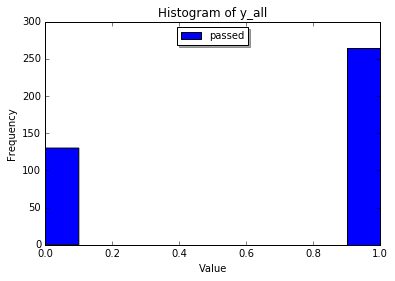
\includegraphics[width=0.5\textwidth]{images/y_all}
  %
\caption{\textbf{Values of `passed' column} \textit{The histograms shows an unbalanced target dataset with approximately 125 values of \{0 - did not pass\} and over 250 values of \{1 - passed\}.}}
\label{y_all}
\end{figure}


\section*{Training and Evaluating Models}
For the student intervention challenge, three supervised learning algorithms have been selected as appropriate learners for the task. The algorithms are as follows:
\begin{enumerate} 
\item Decision Tree Classifier
\item Random Forest Classifier
\item Support Vector Machines
\end{enumerate}



%-------------------------------DECISION TREE CLASSIFIER----------------------------------%

\section*{Decision Tree Classifier}
\begin{itemize} 
\item What is the theoretical $O(n)$ time \& space complexity in terms of input size?\\ 
The theoretical time \& space complexity of decision trees classifiers as implemented in sci-kit learn package is:
\begin{itemize} 
\item Best Case: $\Theta(pN\log^2 N)$ 
\item Worst Case: $O(pN^2\log N)$
\item Average Case: $\Theta(pN\log^2 N)$
\end{itemize}
Where $N$ denotes the number of samples, and $p$ the number of input variables. \footnote{Complexity analysis gotten from Louppe, Gilles PhD dissertation \textit{Understanding Random Forests: From Theory to Practice}, 2014.}

\item What are the general applications of this model?\\
The decision tree algorithm is usually applied to classification and regression problems. They are very popular in operations research, especially for building decision support systems. \\
What are its strengths and weaknesses?\\  

\begin{remark}{Strengths and Weaknesses of Decision Tree Classifiers}
       \begin{itemize}
       \item Strengths of Decision Trees:
              \begin{itemize} 
                     \item Very intuitive. You can look at the results and understand it. 
                     \item Requires little data preparation. 
                     \item The cost of using the tree (i.e., predicting data) is logarithmic in the number of data points used to train the tree. In average case the cost of training $ O(pN\log^2 N)$.
                     \item Able to handle both numerical and categorical data.
                     \item Very robust. Performs well even if its assumptions are somewhat violated by the true model from which the data were generated.
              \end{itemize}
       \item Weaknesses of Decision Trees:
              \begin{itemize} 
                     \item Decision-tree learners can create over-complex trees that do not generalize the data well. They are prone to over-fitting especially in the case of data with lots of features.
                     \item Decision trees can be unstable because small variations in the data might result in a completely different tree being generated. 
                     \item The problem of learning an optimal decision tree is known to be NP-complete under several aspects of optimality and even for simple concepts. 
                     \item There are concepts that are hard to learn because decision trees do not express them easily, such as XOR, parity or multiplexer problems.
                     \item Decision tree learners create biased trees if some classes dominate. 
              \end{itemize}
       \end{itemize}
\end{remark}


\item Given what you know about the data so far, why did you choose this model to apply?\\
The \textit{major} reason why the decision tree classifier was selected was its interpretability. For this problem domain, it isn't just satisfactory to identify students that need intervention, what learning researchers ultimately want is to gain \textit{insights} into the nature of learning, and the social factors that lead to certain outcomes for at-risk students. A decision tree learner, with its ability to graphically plot out the tree becomes a research tool in the hands of learning scientists. Consequently, this can help the school board of supervisors build better solutions for those students which well executed could potentially reduce the costs associated with remediating failed students.\\

\end{itemize} 




%-----------------------------RANDOM FOREST CLASSIFIER---------------------------------------%

\section*{Random Forest Classifier}
\begin{itemize} 
\item What is the theoretical $O(n)$ time \& space complexity in terms of input size?\\
The theoretical time \& space complexity for building a complete unpruned decision tree is:
\begin{itemize} 
\item Best Case: $\Theta(MK\widetilde{N}\log^2 \widetilde{N})$ 
\item Worst Case: $O(MK\widetilde{N}^2\log \widetilde{N})$ 
\item Average Case: $\Theta(MK\widetilde{N}\log^2 \widetilde{N})$
\end{itemize}
Where $M$ denotes number of randomized trees, $N$ the number of samples, and $K$ the number of variables randomly drawn at each node. $\widetilde{N} = 0.632 N$, due to the fact that bootstrap samples draw, on average, $63.2\%$ of unique samples. 
\footnote{Complexity analysis gotten from Louppe, Gilles PhD dissertation \textit{Understanding Random Forests: From Theory to Practice}, 2014.}

\item What are the general applications of this model?\\
Ensemble learners are used in supervised learning. They have multiple applications. They have been used in bioinformatics for example to classify micro-array data, they have been used in engineering to solve aircraft engine fault diagnosis, they have also been used for human pose detection in the Microsoft Kinect amongst other things. \\ 

\item What are its strengths and weaknesses?\\
\begin{remark}{Strengths and Weaknesses of Random Forest Classifiers}
  \begin{itemize} 
       \item Strenghts of Random Forest Classifiers:
              \begin{itemize} 
                     \item Considered one of the best off-the-shelf learning algorithm, requires almost no tuning. 
                     \item Fast to train because algorithm lends itself well to parallelization.
                     \item Flexible, can be used with large number of attributes, small or large datasets.
                     \item Good control of bias and variance because of the averaging and randomization which leads to better performance.
              \end{itemize}
       \item Weaknesses of Random Forest Classifiers:
              \begin{itemize} 
                     \item Loss of interpretability as compared to decision trees.
              \end{itemize}
       \end{itemize}
  \end{remark}


\item Given what you know about the data so far, why did you choose this model to apply?\\
Based on the domain of the dataset, i.e., education and the task itself, identifying students that need intervention, I selected a Random Forest classifier as a potential model because they not only work well in discriminating the data, but these models also lend themselves well as a means of understanding variable importance, i.e., feature selection. Through feature selection, we can come to understand the variables that have the most impact in determining whether a student needs intervention or not.
For example, I trained a Random Forest classifier on the student data, and used its \texttt{feature\_importances\_} function in SciKit learn to find the top 10 most important features in determining when a student needed intervention. Those features are listed below in order of importance : 

\begin{enumerate} 
 \item \textbf{absences} - number of school absences
 \item \textbf{age} - student's age 
 \item \textbf{failures} - number of past class failures
 \item \textbf{goout} - going out with friends
 \item \textbf{Medu} - mother's education
 \item \textbf{Walc} - weekend alcohol consumption
 \item \textbf{health} - current health status
 \item \textbf{Fedu} - father's education
 \item \textbf{freetime} - free time after school
 \item \textbf{studytime} - weekly study time
\end{enumerate}

\end{itemize} 



%-------------------------------------------S V M -----------------------------------------%

\section*{Support Vector Machine (SVMs)}
\begin{itemize}
\item What is the theoretical $O(n)$ time \& space complexity in terms of input size?\\
The theoretical time \& space complexity of SVMs is:
\begin{itemize} 
\item Best Case: $\Theta(pN^2)$ 
\item Worst Case: $O(pN^3)$
\item Average Case: $\Theta(pN^2)$
\end{itemize}
Where $N$ denotes the number of samples, and $p$ the number of input variables. 
It can be a costly algorithm since the compute and storage requirements increase rapidly with the number of training vectors. Even though the algorithm spends more time in training, however, it achieves better $ F_1$ score for prediction as can be seen in table \ref{svmTable}, thus it is more accurate.

\item What are the general applications of this model?\\ 
SVMs are an algorithm used for classification, regression and outlier detection. They are popular in bioinformatics for protein classification. They are also frequently used in text and hypertext classification. \\
What are its strengths and weaknesses?
\begin{remark}{Strengths and Weaknesses of SVMs}
\begin{itemize}
       \item Strenghts of SVMs:
              \begin{itemize} 
                     \item Versatile: utilizes \textbf{kernel} transformation and several functional forms so that what was once non-linearly separable now becomes linearly separable.
                     \item Effective in high dimensional spaces.
                     \item Still effective in cases where number of dimensions is greater than the number of samples.
                     \item Uses a subset of training points in the decision function (called support vectors), so it is also memory efficient.
              \end{itemize}
       \item Weaknesses of SVMs:
              \begin{itemize} 
                     \item If the number of features is much greater than the number of samples, the method is likely to give poor performance.
                     \item SVMs do not directly provide probability estimates, these are calculated using an expensive five-fold cross-validation.
                     \item SVM is a binary classifier. To do a multi-class classification, only pair-wise classifications can be used (one class against all others, for all classes).
              \end{itemize}
       \end{itemize}
\end{remark}

\item Given what you know about the data so far, why did you choose this model to apply?\\
One of the more interesting aspect of this dataset is that it is unbalanced. As previously stated, and can be seen from figure \ref{y_all}, there are more examples of student success than failure. As such, the optimal learner for this problem is one that can still generate reasonable classification given the unbalanced dataset. SVMs are very very robust classifiers and \textit{more importantly}, they have a method of \textit{biasing} the soft-margin constant, $C$, to correct for class imbalances. The solution is to assign a different soft-margin constant to each class.

\end{itemize}

%----------------------------------------------------------------------------------------

\section*{Choosing the Best Model}

\paragraph{\textbf{Question}} Based on the experiments you performed earlier, in 1-2 paragraphs explain to the board of supervisors what single model you chose as the best model. Which model is generally the most appropriate based on the available data, limited resources, cost, and performance?

\paragraph{\textbf{Answer}} In determining which model best fits the job for identifying students that need intervention, we start off by looking at the model that gives the best performance based on accuracy. Looking at our three tables---table \ref{decisionTreeTable}, table \ref{randomForestClassifierTable}, and table \ref{svmTable}---we can see that the learner that gives the best performance is the \textbf{Support Vector Machine}(SVM). This learner gives 11.2\% improvement over the Decision Tree model, as well as a 2.8\% performance improvement over the Random Forest model.

From table \ref{decisionTreeTable}, we can see that the decisionTree classifier has over-fitted the training data, giving a $F_1$ of 1.00, even though it has the shortest training and prediction time. True to the ensemble methods claim of prevent over-fitting, the Random Forest classifier, doesn't over-fit the data and greatly improves its performance over the Decision tree model. However, it doesn't out compete an SVM for this problem.

In conclusion, for the problem of identifying students that need intervention, I would advice the board of supervisors to go with a \textbf{Support Vector Machine}. First, it is a relatively fast algorithm to train and predict. Second, as we can see from figure \ref{y_all}, the dataset is quite unbalanced (number of passed students $>>$ number of failed students) and relatively small. The SVM algorithm is able to handle this better than the other two models. This model does take the longest to train, but that is something the board will not be doing all the time. Instead, the board will need to constantly run the prediction algorithm. While its marginally slower in prediction than Random Forest classifier with a prediction time of 0.002 seconds versus 0.001 seconds as can be seen from tables \ref{randomForestClassifierTable} and \ref{svmTable}. The difference of negligible and SVM makes up for what it loses in speed with improvement in accuracy.


\paragraph{\textbf{Question}} In 1-2 paragraphs explain to the board of supervisors in layman's terms how the final model chosen is supposed to work (for example if you chose a Decision Tree or Support Vector Machine, how does it make a prediction).

\paragraph{\textbf{Answer}} A Support Vector Machine is a class of discriminatory algorithms. The goal is to try and correctly classify a dataset into separate classes. Subject to that constraint, an SVM  picks a decision boundary that separates the classes by maximizing the distance to the nearest points in either classes. These points are a subset of the dataset and are called support vectors. 


\begin{figure}[!hbtp]
\centering
    \subfloat[Features in two dimensional space.]{%
    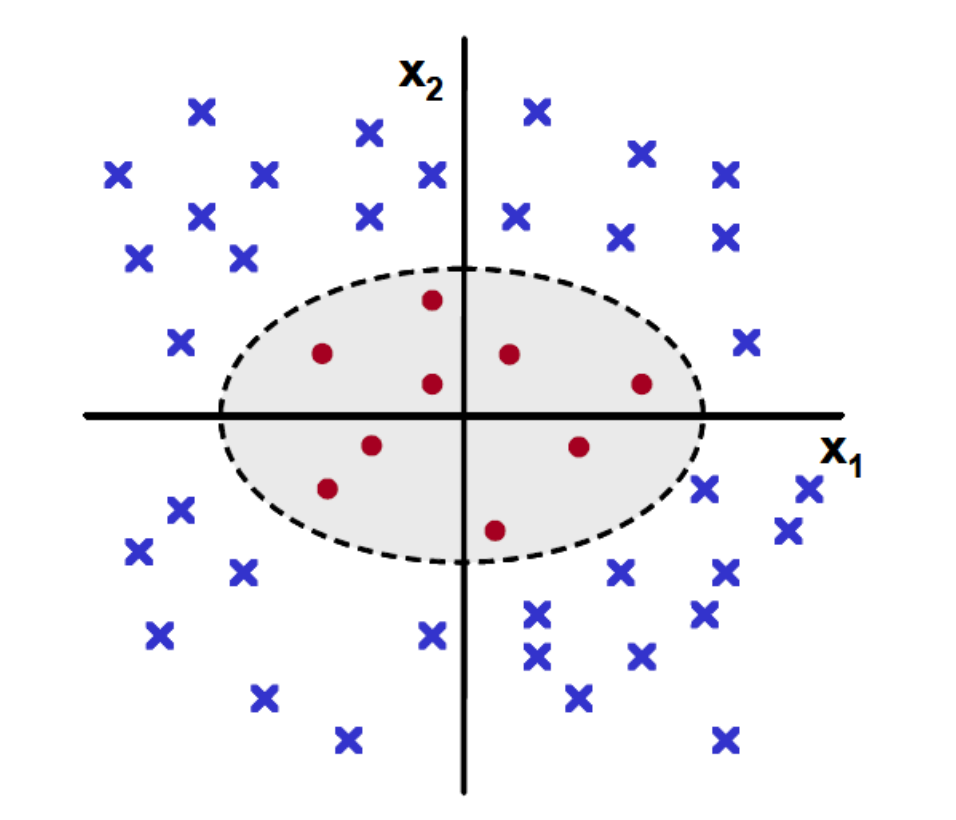
\includegraphics[width=0.5\textwidth]{images/SVMNonlinear1}
    \label{SVMNonlinear1}}
    \subfloat[Features projected in three dimensional space.]{%
    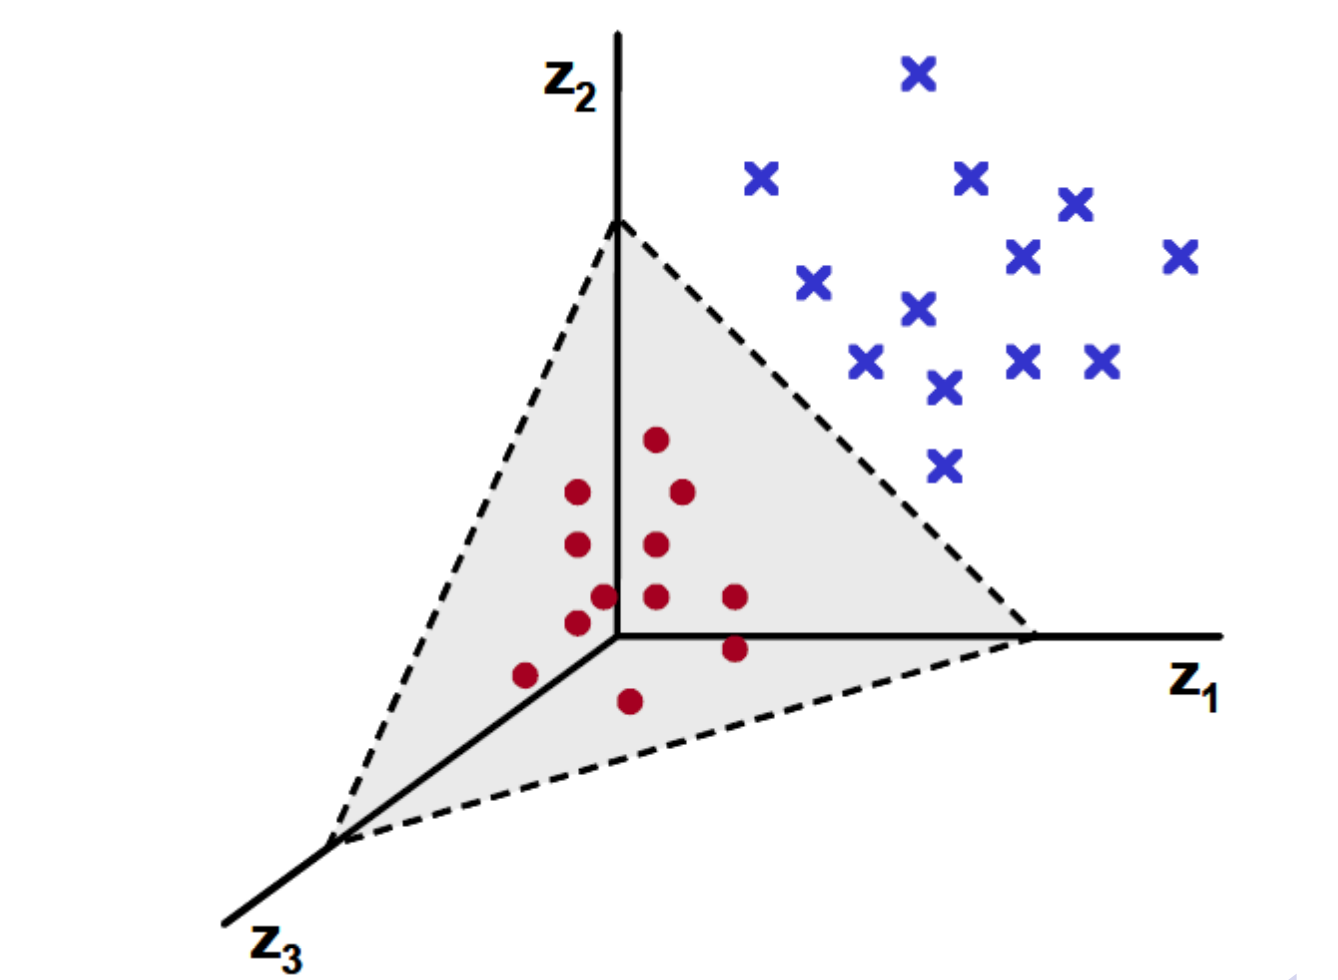
\includegraphics[width=0.5\textwidth]{images/SVMNonlinear2}
    \label{SVMNonlinear2}}
    \caption{\textbf{Kernel trick.} \textit{Figure (a) $\vec{x} = \{x_1,x_2\}$. Figure (b) $\vec{z}$ by $\vec{x} = \{x_1,x_2\} \longrightarrow \vec{z} = \{x_1^2, \sqrt2x_1x_2, x_2^2 \}$. By mapping the data from two dimensions to three dimension, the data now becomes linearly separable in the new representation.}}
\end{figure}

The most interesting thing about SVMs is what is know as the \textit{kernel} trick. This procedure make linear models work in nonlinear settings by mapping the data into higher dimensions where we can see the linear behavior. For example, figure \ref{SVMNonlinear1} shows a data in two-dimensional space where it is evident we will not be able to find a decision boundary that separates the data into two classes. Using a kernel, the features are projected into a three dimension space as is shown in figure \ref{SVMNonlinear2}. In this space, we can find a hyperplane that will linearly separate the data into two classes. This aspect of SVMs is what makes them really robust.

An SVM does prediction on the data by classifying the test dataset based on the decision boundary it ``fitted'' during its training phase. There are several evaluation metrics that let you determine the accuracy of the algorithm.


\paragraph{\textbf{Question}} Fine-tune the model. What is the model's final $F_1$ score?
\paragraph{\textbf{Answer}} As it is often done in practical machine learning, we try several kernels first, often the linear kernel, then the RBF kernel. Using the linear kernel, the $C$ hyper-parameter was tuned with the following values: $ \{2^{-5}, 2^{-4}, 2^{-3}, 2^{-2}, 2^{-1}, 2^{-0}, 2^{1} \}$. Figure \ref{tunedC} shows the results of trying various $C$ with gridsearch. 


\begin{figure}[!htbp]
  \centering
    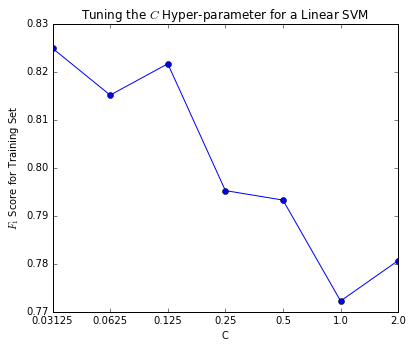
\includegraphics[width=0.8\textwidth]{images/C_Hyperparameter}
  %
\caption{\textbf{Values of $F_1$ scores for different values of $C$.} \textit{From this figure, we can see that we achieve the highest value of $F_1$ where $C$ = 0.03125}}
\label{tunedC}
\end{figure}




\setlength{\extrarowheight}{1.5pt}
\begin{table}[!htbp]
\caption{Result of tuning with \textbf{GridSearchCV}} %title of the table
\centering % centering table
\begin{tabular}{|p{4cm}||p{4cm}|} % creating four columns
\hline % inserts single-line
& GridSearchCV\\[0.5ex]
\hline % inserts single-line

F1 score for training set     &0.831\\
F1 score for test set         &0.795\\

\hline % inserts single-line 
& Best Parameters \\[1ex]
\hline % inserts single-line

Kernel & Linear\\
$C$ & 0.03125\\
\hline % inserts single-line
\end{tabular}
\label{tunedGridSearch}
\end{table}








%-------------------------------------------T A B L E S-----------------------------------------%

\section*{Tables}

\setlength{\extrarowheight}{1.5pt}
\begin{table}[!htbp]
\caption{Result of training with a \textbf{DecisionTreeClassifier}} %title of the table
\centering % centering table
\begin{tabular}{|p{6cm}|p{1.5cm}|p{1.5cm}|p{1.5cm}|} % creating four columns
\hline % inserts single-line
& \multicolumn{3}{c|}{Training set size}\\[5pt]
\cline{2-4} 
& 100 & 200 & 300\\[0.5ex]
\hline % inserts single-line

Training time (secs)          &  0.001&  0.001&  0.002\\ 
Prediction time (secs)        &  0.000&  0.000&  0.000\\ 
F1 score for training set     &  1.000&  1.000&  1.000\\ 
F1 score for test set         &  0.603&  0.716&  0.672\\

\hline % inserts single-line
\end{tabular}
\label{decisionTreeTable}
\end{table}

\setlength{\extrarowheight}{1.5pt}
\begin{table}[!htbp]
\caption{Result of training with a \textbf{Random Forest Classifier}} %title of the table
\centering % centering table
\begin{tabular}{|p{6cm}|p{1.5cm}|p{1.5cm}|p{1.5cm}|} % creating four columns
\hline % inserts single-line
& \multicolumn{3}{c|}{Training set size}\\[5pt]
\cline{2-4} 
& 100 & 200 & 300\\[0.5ex]
\hline % inserts single-line

Training time (secs)          &  0.034&  0.037&  0.020\\ 
Prediction time (secs)        &  0.003&  0.001&  0.001\\ 
F1 score for training set     &  1.000&  0.996&  0.995\\ 
F1 score for test set         &  0.740&  0.818&  0.756\\ 
\hline % inserts single-line
\end{tabular}
\label{randomForestClassifierTable}
\end{table}


\setlength{\extrarowheight}{1.5pt}
\begin{table}[!htbp]
\caption{Result of training with a \textbf{SVMs}} %title of the table
\centering % centering table
\begin{tabular}{|p{6cm}|p{1.5cm}|p{1.5cm}|p{1.5cm}|} % creating four columns
\hline % inserts single-line
& \multicolumn{3}{c|}{Training set size}\\[5pt]
\cline{2-4} 
& 100 & 200 & 300\\[0.5ex]
\hline % inserts single-line

Training time (secs)          &  0.001&  0.004&  0.008\\ 
Prediction time (secs)        &  0.001&  0.001&  0.002\\ 
F1 score for training set     &  0.878&  0.868&  0.876\\ 
F1 score for test set         &  0.775&  0.781&  0.784\\
\hline % inserts single-line
\end{tabular}
\label{svmTable}
\end{table}


\end{document}  